\documentclass[12pt]{article}
\linespread{1.2}
\usepackage[margin=2cm]{geometry}
\usepackage[utf8]{inputenc}
\usepackage{amsfonts}
\usepackage{amsmath}
\usepackage{multicol}
\usepackage{amsthm}
\usepackage{amssymb,scrextend}
\usepackage{graphicx,tikz}
\newtheorem{dfn}{Definition}
\renewcommand{\qed}{\hfill$\blacksquare$}
\let\newproof\proof
\renewenvironment{proof}{\vspace{1em}\begin{addmargin}[2em]{0em}\begin{newproof}}{\end{newproof}\end{addmargin}\qed}
\newenvironment{theorem}[2][Theorem]{\begin{trivlist}
\item[\hskip \labelsep {\bfseries #1} \hskip \labelsep {\bfseries #2.}]}{\end{trivlist}}
\newenvironment{example}[2][Example]{\begin{trivlist}
\item[\hskip \labelsep {\bfseries #1} \hskip \labelsep {\bfseries #2.}]}{\end{trivlist}}
\newenvironment{lemma}[2][Lemma]{\begin{trivlist}
\item[\hskip \labelsep {\bfseries #1} \hskip \labelsep {\bfseries #2.}]}{\end{trivlist}}
\newenvironment{exercise}[2][Exercise]{\begin{trivlist}
\item[\hskip \labelsep {\bfseries #1} \hskip \labelsep {\bfseries #2.}]}{\end{trivlist}}
\newenvironment{problem}[2][Problem]{\begin{trivlist}
\item[\hskip \labelsep {\bfseries #1} \hskip \labelsep {\bfseries #2.}]}{\end{trivlist}}
\newenvironment{corollary}[2][Corollary]{\begin{trivlist}
\item[\hskip \labelsep {\bfseries #1} \hskip \labelsep {\bfseries #2.}]}{\end{trivlist}}
\usepackage{fancyhdr,enumitem,changepage,url}
\pagestyle{fancy}
\author{Warren Atkison}
\date{\today}
\setlength{\headheight}{15pt}
\begin{document}
\fancyhf{}
\fancyhead[L]{Warren Atkison}
\fancyhead[C]{Homework Set 6}
\fancyhead[R]{\today}
\fancyfoot[R]{\thepage}

\begin{exercise}{5.1.13 (3pt)}
	Prove a sequence $d_1 \ge d_2 \ge \ldots \ge d_n$ is graphical if $\sum_{i=1}^n d_i$ is even and for all $k \in \{1,2,\ldots,n\}$,
	\[
		\sum_{i=1}^k d_i \le  k(k-1) + \sum_{i=k+1}^n \min(d_i,k).
	\]
\end{exercise}
\begin{proof}
	Induction on $s = \sum_{i=1}^n d_i$. This is easy to see when $s = 2$, so suppose $s > 2$. WLOG, let $d_n > 0$. Let $t$ be the least integer such that $d_t > d_{t+1}$, or $t=n-1$ if there is no such integer. Let $d'_t = d_t - 1$, $d'_n = d_n - 1$, and $d'_i=d_i$ for all other $i$. Note that $d'_1 \ge d'_2 \ge \ldots \ge d'_n$. We want to show that $\{d'_i\}$ satisfies the condition of the theorem that for all $k \in \{0,\ldots,n\}$
	\[
		\sum_{i=1}^k d'_i \le k(k-1) + \sum_{i=k+1}^n \min(d'_i,k)
	\]
	of which there are five cases:
	\begin{itemize}
		\item[1.] $k \ge t$. Note that $\min(a,b) - 1 \le \min(a-1,b)$. When $k < n$.
			\begin{align*}
				\sum_{i=1}^k d'_i &= \sum_{i=1}^k d_i - 1 \\
						  &\le k(k+1) + \sum_{i=k+1}^n \min(d_i,k) - 1 \\
						  &= k(k+1) + \sum_{i=k+1}^{n-1} \min(d'_i,k) + \min(d_n,k) - 1 \\
						  &\le k(k+1) + \sum_{i=k+1}^{n-1} \min(d'_i,k) + \min(d_n - 1,k) \\
						  &= k(k+1) + \sum_{i=k}^{n} \min(d'_i,k)
			\end{align*}
		\item[2.] $k < t,d_k < k$. Note that $d_k \le k - 1$
			\begin{align*}
				\sum_{i=1}^k d'_i &= kd_k \le k(k-1) \le k(k-1) + \sum_{i=k+1}^{n} \min(d'_i,k)
			\end{align*}
		\item[3.] $k < t,d_k = k$. Consider $d_{k+2} + d_{k+3} + \ldots + d_n$. If $k < n - 2$, then we have
			\[
				\ldots + d_{n-1} + d_n \ge 2
			\]
			since $d_{n-2} \ge d_n \ge 1$. If $k \ge n - 2$, then $t = n - 1$, and our minimum case for our sequence ($d_i = d_k = k = n-2$ for $1\le i < n$) is
			\[
				\{d_i\} = (n-2), (n-2), \ldots, d_n.
			\]
			But then, $s = (n-1)(n-2) + d_n$ must be even, so $d_n$ must be even and therefor $d_n \ge 2$. Also, since $k<t$ we have $d_i = d_k = k$ for $1 \le i \le k+1$, so
			\begin{align*}
				\sum_{i=1}^k d'_i = kd'_k = k^2 - k + k &= k^2 - k + d_{k+1} \\
									&\le k(k-1) + d_{k+1} + d_{k+2} + \ldots d_n - 2 \\
									&\le k(k-1) + \sum_{i=k+1,i\neq t}^{n-1} \min(d_i,k) + d_t - 1 + d_n - 1 \\
									&= k(k-1) + \sum_{i=k+1,i\neq t}^{n-1} \min(d'_i,k) + d'_t + d'_n \\
									&\le k(k-1) + \sum_{i=k+1}^n \min(d'_i,k)
			\end{align*}
		\item[4.] $k < t,d_n > k$. Then $\min(d_i,k) = \min(d_i-1,k) = k$ for all $1 \le i \le n$, so
			\begin{align*}
				\sum_{i=1}^n d'_i &= \sum_{i=1}^n d_i \\
						  &\le k(k+1) + \sum_{j=k+1}^n \min(d_i,k) \\
						  &\le k(k+1) + \sum_{j=k+1}^n \min(d'_i,k)
			\end{align*}
		\item[5.] $k < t,d_k > k, d_n \le k$
			\[
				\ldots
			\]
	\end{itemize}
	So $\{d'_i\}$ satisfies the if part of the theorem. By induction, we can assume $\{d'_i\}$ is graphical. Let $G$ be the graph formed by $\{d'_i\}$ with vertices $v_1,v_2,\ldots,v_n$. If there is no edge between $v_t$ and $v_n$, then we can add this edge to $G$ and this appended graph has degree sequence $\{d_i\}$. Otherwise, we are still 2 edges short, so there exists some $v_i$ where $v_t$ and $v_m$ have no edge. Also, since $d_i \ge d_n$, there is some $v_j$ where $v_i$ and $v_j$ share an edge, and $v_j$ and $v_n$ don't. We can remove the edges from $v_t$ to $v_n$ and $v_i$ to $v_j$, and add the edges $v_i$ to $v_t$ and $v_j$ to $v_n$ to get another graph $G'$ formed by $\{d'_i\}$ without edges from $v_t$ to $v_n$. $G'$ is still of degree sequence $\{d'_i\}$, so adding the edge from $v'_t$ to $v'_n$ gives us a graph with degree sequence $\{d_i\}$
	
\end{proof}

Note: I ended up using the proof by S.A. Choudum as an outline which was referenced in the textbook. Since it was referenced I figured this was okay, but I still tried to state each step as I understood it and fill in some gaps the Choudum found trivial. There are some things about the proof I still have questions on, mainly on the 5th case but for the most part sifting through this elegant proof was very interesting.

\begin{exercise} {5.1.2 (2pt)}
	Prove that if $\sum_{i=1}^n d_i$ is even, there is a graph with degree sequence $d_1,d_2,\ldots,d_n$.
\end{exercise}
\begin{proof}
	Induction on $n$. When $n=1$, $d_1$ must be even, so we can form a graph with one vertex and with deg$(d_1)/2$ loops. Let $\sum_{i=1}^n d_i$ be even, and $G$ be a graph with degree sequence $\{d_i\}$.  Now let $\sum_{i=1}^{n+1} d_i$ be even.

	Suppose $d_{n+1}$ is even, then $\sum_{i=1}^n d_i$ must be even and by our inductive hypothesis form a graph $G$. Let $G'$ be a new graph. Since $d_{n+1}$ is even, we can add vertex to $G'$ with deg$(d_{n+1})/2$ loops, and then add the graph all vertices and edges from $G$ to form a graph with the sequence $d_1,d_2,\ldots,d_{n+1}$.

	Now suppose $d_{n+1}$ is odd, then $\sum_{i=1}^n d_{i}$ must be odd. From the sequence $d_1, d_2, \ldots, d_n$, choose some $d_i$ for $1 \le i \le n$ and let $d'_i = d_i - 1$. Then the sequence $d_1, d_2, \ldots,d'_i,\ldots,d_n$ is even and forms a graph $G$. Let $G'$ be a new graph. add a vertex with deg$(d_{n+1} - 1)/2$ loops add all vertices and edges from $G$ to $G'$. Finally add one edge from the vertex with degree $d'_i$ to $d_{n+1}$ to form a graph of sequence $d_1,d_2,\ldots,d_{n+1}$.
\end{proof}
\begin{exercise} {5.1.3 (2pt)}
	Suppose $d_1 \ge d_2 \ge \ldots \ge d_n$ and $\sum_{i=1}^n d_i$ is even. Prove that there is a multi-graph (no loops) with degree sequence $d_1,d_2,\ldots,d_n$ if and only if $d_1 \le \sum_{i=2}^n d_i$.
\end{exercise}
\begin{proof}
	Induction on $s = \sum_{i=1}^n d_i$. When $s = 0$ this is trivial, when $s = 2$ we have $d_1 = 1 = d_k$ for some $2 \le k \le n$ and $d_i = 0$ for $i \neq k$ and $2 \le i \le n$ ($n$ vertices with one edge between two points). Now let $d_1 \ge d_2 \ge \ldots \ge d_n$, $\sum_{i=1}^n d_i = s$ and the degree sequence $d_1,d_2,\ldots,d_n$ form a loop-less graph $G$. Now let $d'_{1} \ge d'_{2} \ge \ldots \ge d'_n$ and $\sum_{i=1}^n d'_i = s + 2$.

	Suppose $d'_1 = \sum_{i=2}^n$. Then we can draw a graph with vertices $v_1,v_2,\ldots,v_n$. From $v_1$ to $v_2$, draw $d'_2$ edges, from $v_1$ to $v_3$, draw $d'_3$ edges, and etc. This gives us a loop-less graph with the desired degree sequence.

	Suppose $d'_1 < \sum_{i=2}^n$. Because $d'_1$ is the greatest value in the sequence, there must be two non-zero $d'_j$ and $d'_k$ such that $1 \le j < k \le n$. Then, $\sum_{i=1,i\neq i,j}^n d'_i + d_k - 1 + d_j - 1 = s$, so then there is a loop-less graph $G$ with degree sequence $d'_1,d'_2,\ldots,d'_j - 1,\ldots,d'_k-1,\ldots,d'_n$. Let $G'$ be a new graph with the same vertices and edges as $G$, but with a extra edge between the vertices with degree $d'_j - 1$ and degree $d'_k - 1$. This gives us a loop-less graph with the desired sequence.
\end{proof}
\begin{exercise} {5.2.3 (2pt)}
	Prove that if vertices $v$ and $w$ are joined by a walk they are joined by a path.
\end{exercise}
\begin{proof}
	Construction. Let $W = \{v_1,e_1,v_2,e_2,\ldots,v_k,e_k,v_{k+1}\}$ form a walk. We can give an algorithm with a finite amount of steps that given $W$ will return a path $P$. Since a walk is also a graph, and $v_1$ is connected to $v_{k+1}$ by definition, we can always take the shortest path in our graph given by the walk from $v_1$ to $v_k$. Attached to this assignment is a python script which given a walk/graph, it generates all possible walks of a certain length and finds a path (using depth first search). Here is the demo graph I included in the script
\end{proof}
\begin{center}
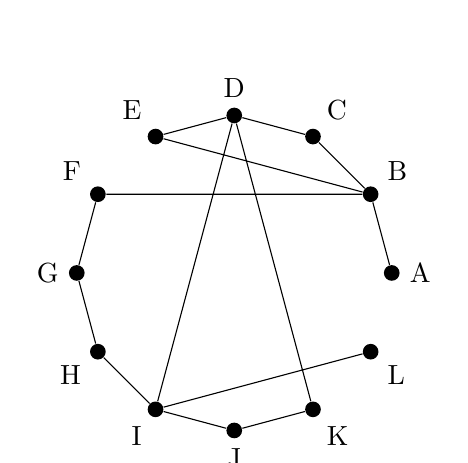
\begin{tikzpicture}[
    vertex/.style={circle, fill, inner sep=2pt}, scale = 1
]
    % Define vertices on a 12-sided polygon
    \foreach \i/\label in {0/A, 30/B, 60/C, 90/D, 120/E, 150/F, 180/G, 210/H, 240/I, 270/J, 300/K, 330/L} {
        \node[vertex, label={\i:\label}] (V\label) at (\i:2) {};
    }
    % Connect vertices with edges (optional)
    \draw (VA) -- (VB) -- (VC) -- (VD) -- (VE) -- (VB) -- (VF) -- (VG) -- (VH) -- (VI) -- (VJ) -- (VK) -- (VD) -- (VI) -- (VL);
\end{tikzpicture}
\end{center}

\begin{exercise} {5.3.3 (2pt)}
	The graph shown below is the Peterson graph. Does it have a Hamilton cycle? Does it have a Hamilton path?
\end{exercise}
\begin{center}	

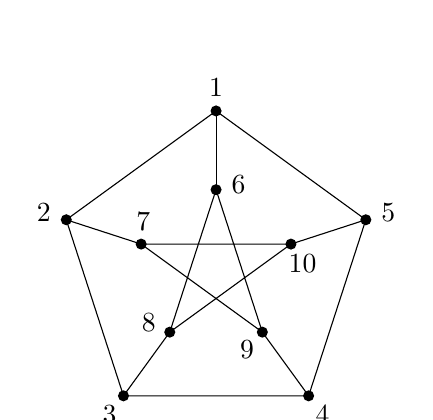
\begin{tikzpicture}[scale=1]
    % Define vertices
    \foreach \i in {0,...,4} {
        \coordinate (V\i) at (90 + 72*\i:2);
        \coordinate (W\i) at (90 + 72*\i:1);
    }

    \foreach \i/\num/\deg/\wnum in {0/1/72/6,1/2/144/7,2/3/216/8,3/4/288/9,4/5/360/10} {

	\fill (V\i) circle (2pt) node at (\deg + 18:2.3) {\num};
	\fill (W\i) circle (2pt) node at (\deg + 3:1.1) {\wnum};
    }

    \draw (V0) -- (V1) -- (V2) -- (V3) -- (V4) -- (V0);
    \draw (W0) -- (W2) -- (W4) -- (W1) -- (W3) -- (W0);

    \foreach \i in {0,...,4} {
	    \draw (V\i) -- (W\i);
    }

\end{tikzpicture}
\end{center}

The Peterson graph has 10 vertices and 15 edges, and has no cycles less than 5. A Hamiltonian cycle needs at least as many edges as vertices, which we have, but then we have an extra 5 left over. With only 5 more edges, we can only construct cycles less than 5, so that Peterson graph has no Hamiltonian cycles. However, there is a Hamilton path, namely
\[
	(1) \to (2) \to (3) \to (8) \to (6) \to (9) \to (4) \to (5) \to (10) \to (7)
\]
\begin{exercise} {5.1.4 (1pt)}
	Prove that 0,1,2,3,4 is not graphical.
\end{exercise}
\begin{proof}
	If there are 5 vertices and one must have degree 4, then no vertex can have degree 0 as the vertex of degree 4 would be connected to the rest of the vertices.
\end{proof}
\end{document}

